\documentclass[class=report,crop=false, 12pt]{standalone}
\usepackage[screen]{../scratch}

\begin{document}


\titre[E]{Variables et hasard}
%===============================


\begin{enigme}

On lance deux dés un grand nombre de fois.
On compte combien de fois la somme des deux dés fait $5$ ou $9$.




\bigskip

\textbf{Question.} J'ai effectué $10\,000$ lancers de mes deux dés. Combien de fois environ ai-je obtenu $5$ ou $9$ :
$1000$ fois, $2000$ fois, $3000$ fois,\ldots, $9000$ fois ou $10\, 000$ fois ?

\bigskip
\emph{Indications.}
\begin{itemize}
  \item Pour chaque lancer d'un dé, on tire au hasard un nombre entre $1$ et $6$.
  \item Le mode turbo permet d'aller plus vite !
\end{itemize}



%\begin{solution}
%Probabilité que la somme soit $5$ : $4/36$ ; probabilité que la somme soit $9$ : $4/36$.
%Donc probabilité $5$ ou $9$ est $8/36 = 2/9 \simeq 0,22$.
%Donc pour $10000$ lancers, environ $2200$ devraient être comptés !
%
%\textbf{Réponse attendue : 2000.}
%\end{solution}

\end{enigme}






\begin{enigme}

Voici une façon de simuler le hasard par ordinateur.

\begin{itemize}
  \item On part d'un entier $x_0$, la \og graine \fg{}.
  \item On calcule un entier $x_1$ en fonction de $x_0$.
  \item On calcule $x_2$ en fonction de $x_1$.
  \item \ldots
\end{itemize}

Si la fonction qui permet de faire les calculs est bien choisie alors les nombres $x_1$, $x_2$, $x_3$... ont l'air d'être tirés au hasard.

Voici l'algorithme que j'utilise :
\begin{itemize}
  \item $x \leftarrow 13$
  \item Répéter $10$ fois :
  \begin{itemize}
    \item $x \leftarrow 11 \times x + 3$
    \item $x \leftarrow x \text{ modulo } 100$
  \end{itemize}
\end{itemize}  

\bigskip

La graine est $13$. Le premier nombre généré est $46$, le second est
$9$, le troisième est $2$... 

\textbf{Question.} Combien vaut le dixième nombre généré ?

\bigskip

\emph{Indications.}
\begin{itemize}
  \item L'opération \og $x \text{ modulo } 100$ \fg{} est une façon simple de garder seulement les deux derniers chiffres de l'entier $x$. Par exemple \og $1234 \text{ modulo } 100$  \fg{} vaut $34$.
  \item Une autre façon, plus mathématique, de définir l'opération \og $x \text{ modulo } 100$ \fg{} est de dire que ce nombre est le reste de la division de $x$ par 100.
  \item On l'obtient avec Scratch par le bloc :
\begin{center}
  
\includegraphics[scale=\scalebloc]{bloc-06-eg2} 
\end{center}  
\end{itemize}

%\begin{solution}
%C'est $93$.
%\end{solution}


\end{enigme}





\begin{enigme}


On lance au hasard des points dans un carré. On compte ceux qui tombent dans le disque délimité par le cercle en rouge (figure de gauche). Sur la figure de droite, on a lancé de nombreux points. En rouge ce sont les points qui sont tombés dans le disque, les autres sont en noir.

\begin{center}
\begin{minipage}{0.49\textwidth}
\myfigure{1.1}{
\tikzinput{montecarlo}
}
\end{minipage}
\begin{minipage}{0.49\textwidth}
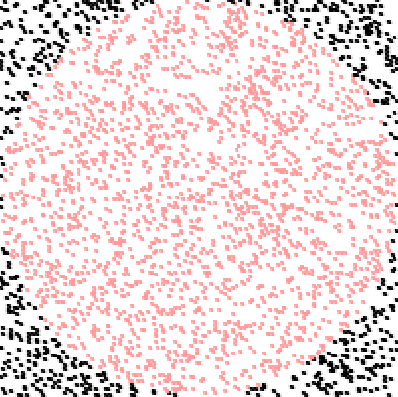
\includegraphics[scale=\scaleecran]{ecran-06-eg3bis} 
\end{minipage}
\end{center}

\bigskip

Comment tirer un point au hasard ?
\begin{itemize}
  \item Tirer au hasard un nombre $x$ entre $-100$ et $+100$.
  \item Tirer au hasard un nombre $y$ entre $-100$ et $+100$.
  \item Le point au hasard est alors $(x,y)$.
\end{itemize}

\bigskip

Comment savoir si le point est bien dans le disque ?
Le point $(x,y)$  est dans le disque lorsque :
$$x \times x + y \times y \le 10\,000.$$

  


\bigskip

\textbf{Question.} On tire beaucoup de points (au moins $5000$).
Combien vaut le nombre :
$$40 \times \frac{\text{nombre de points lancés figurant dans le disque}}{\text{nombre total de points lancés}} \quad ?$$

Pour la réponse, on arrondira à l'entier le plus proche.

\bigskip


%\begin{solution}
%Le rapport est proche $10 \pi$, donc la réponse attendue est $31$.
%\end{solution}

\end{enigme}


\end{document}

